% DESENVOLVIMENTO
% ---- ---- ---- ---- ---- ---- ---- ---- ----
\section{DESENVOLVIMENTO}

% ---- ---- ---- ---- ---- ---- ---- ---- ----
% ---- 2..1 ---- ---- ---- ---- ---- ---- ----
% ---- ---- ---- ---- ---- ---- ---- ---- ----
\subsection{Obter a resposta dada um entrada senoidal}

Um sistema $G_1(s)$ é dado pela \autoref{eq:eq1}, onde m = 500, b = 1000, k = 25000. Para um entrada senoidal de 5 rad/s é obtido uma resposta conforme a Figura~\ref{fig:f1}.
\\
\begin{equation}
    G_1(s) = \frac{ms + b}{m^{2} + bs + k} = \frac{500s + 1000}{500s^{2} + 1000s + 25000}
    \label{eq:eq1}
\end{equation}

\begin{figure}[h!]
    \centering
    \caption{Resposta de $G_1(s)$ a entrada senoidal}
    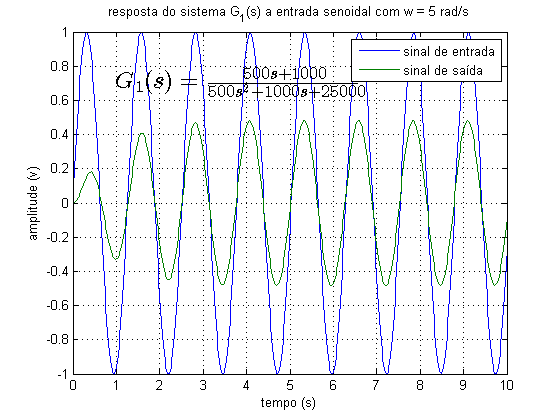
\includegraphics[scale=0.55]{img/task_7_01.png}
    \label{fig:f1}
    \begin{flushleft}
    Fonte: Elaboração própria (2018).
    \end{flushleft}
\end{figure}

Avaliando a amplitude dos dois sinais em regime permanente pode ser determinado a relação de ganho e diferença de fase, que são respectivamente: 0.4822, 0.1000.
Com o auxilio da função \textit{freqresp}, foi avaliado a magnitude e fase para 5 rad/s que são respectivamente: 0.4817, 0.0831.

Frisando que o retorno da função \textit{freqresp} é um número complexo, número este que é a avaliação da função transferência (FT) passada para uma frequência específica. Por exemplo, para $G_1(s)$ em 5 rad/s tem-se como retorno 0.4800 + 0.0400i.

% ---- ---- ---- ---- ---- ---- ---- ---- ----
% ---- 2..2 ---- ---- ---- ---- ---- ---- ----
% ---- ---- ---- ---- ---- ---- ---- ---- ----
\subsection{Analisar um sistema de 2ª ordem sem amortecimento}

Um sistema $G_2(s)$ é dado pela \autoref{eq:eq2}. A resposta a uma entrada senoidal na frequência de ressonância é apresentado na \autoref{f2}. Como era esperado, para tal frequência a saída tende ao infinito.
\\
\begin{equation}
    G_2(s) = \frac{1}{s^{2} + 5}
    \label{eq:eq2}
\end{equation}

\begin{figure}[h!]
    \centering
    \caption{Resposta de $G_2(s)$ na frequência ressonante}
    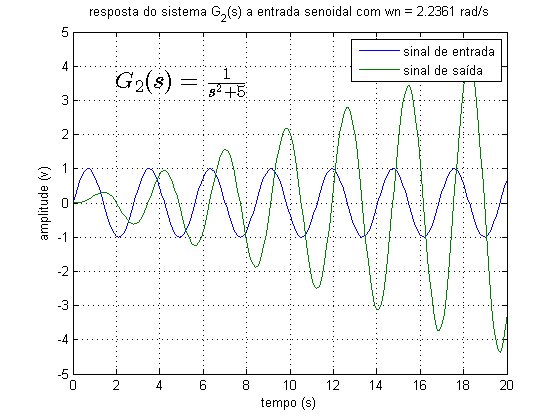
\includegraphics[scale=0.55]{img/task_7_02.png}
    \label{f2}
    \begin{flushleft}
        Fonte: Elaboração própria (2018).
    \end{flushleft}
\end{figure}

% ---- ---- ---- ---- ---- ---- ---- ---- ----
% ---- 2..3 ---- ---- ---- ---- ---- ---- ----
% ---- ---- ---- ---- ---- ---- ---- ---- ----
\subsection{Obter a resposta dada um entrada senoidal para diferentes frequências}

Na tentativa de gerar subsídios para melhor avaliar um sistema, foi variado a frequência natural para o sistema $G_2(s)$ e visualizado a resposta no tempo dada uma entrada senoidal, conforme a \autoref{f3}
\\
\begin{figure}[h!]
    \centering
    \caption{Resposta de $G_2(s)$ para diferentes frequências}
    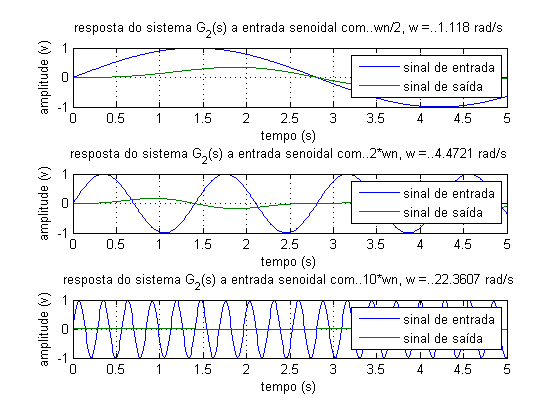
\includegraphics[scale=0.55]{img/task_7_03.png}
    \label{f3}
    \begin{flushleft}
        Fonte: Elaboração própria (2018).
    \end{flushleft}
\end{figure}

E complementando os dados anteriores, foi visualizado a resposta na frequência, conforme a \autoref{f4}. Essa resposta da amplitude em função da frequência é o princípio do diagrama de bode
\\
\begin{figure}[h!]
    \centering
    \caption{Resposta na frequência de $G_2(s)$}
    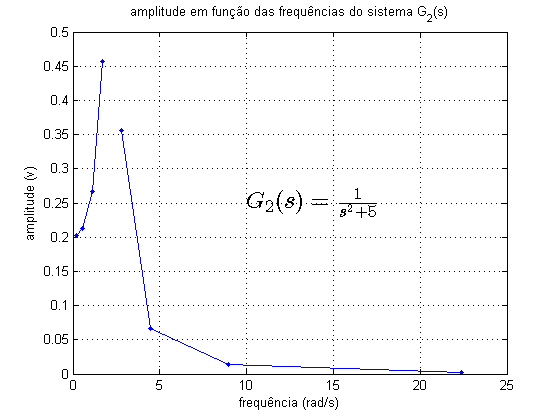
\includegraphics[scale=0.55]{img/task_7_04.png}
    \label{f4}
    \begin{flushleft}
        Fonte: Elaboração própria (2018).
    \end{flushleft}
\end{figure}

% ---- ---- ---- ---- ---- ---- ---- ---- ----
% ---- 2..4 ---- ---- ---- ---- ---- ---- ----
% ---- ---- ---- ---- ---- ---- ---- ---- ----
\subsection{Diagrama de Bode}
Ainda analisando o sistema de $G_2(s)$ foi coletado o diagrama de Bode do mesmo, conforme a \autoref{f5}.

\begin{figure}[h!]
    \centering
    \caption{Diagrama de bode de $G_2(s)$}
    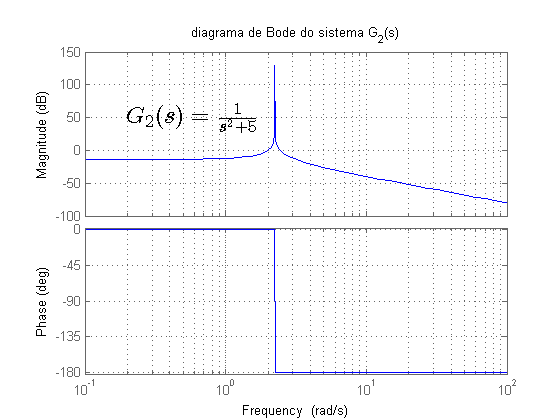
\includegraphics[scale=0.55]{img/task_7_05.png}
    \label{f5}
    \begin{flushleft}
        Fonte: Elaboração própria (2018).
    \end{flushleft}
\end{figure}

Outras duas informações coletas foram o nível contínuo, e a primeira frequência onde foi apresentado uma relação de \textit{3dB}. Para obter o nível contínuo foi utilizado a função \textit{dcgain}, onde o retorno foi 0.2. E para obter o a primeira frequência com \textit{3dB} foi utilizado a função \textit{bandwith}, onde o retorno foi 3.4731.

% ---- ---- ---- ---- ---- ---- ---- ---- ----
% ---- 2..5 ---- ---- ---- ---- ---- ---- ----
% ---- ---- ---- ---- ---- ---- ---- ---- ----
\subsection{Análise em função da varição de parâmetros}
Um sistema $G_3(s)$ é dado pela \autoref{eq:eq3}, onde as variáveis m e k são fixas, m = 1, k = 5.
\\
\begin{equation}
    G_3(s) = \frac{1}{m^{2} + bs + k} = \frac{1}{s^{2} + bs + 5}
    \label{eq:eq3}
\end{equation}
\\\indent
Variando b pode-se avaliar de forma mais pontual a influência dessa componente. Para tal foi variado b com os seguintes valores: 0.1, 0.5, 0.8, 1, 2 e 4. A resposta desse diagrama de Bode é apresentado na \autoref{f6}.
 \\
\begin{figure}[h!]
    \centering
    \caption{Diagrama de Bode de $G_3(s)$}
    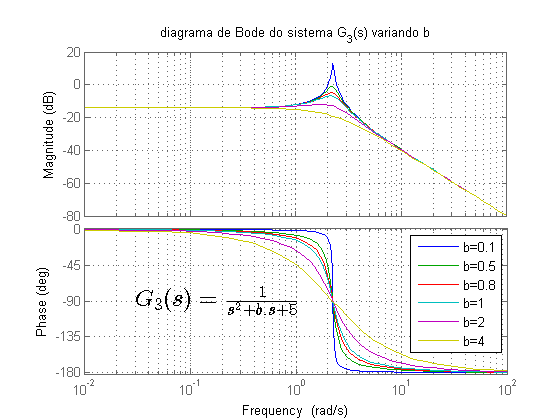
\includegraphics[scale=0.55]{img/task_7_06.png}
    \label{f6}
    \begin{flushleft}
        Fonte: Elaboração própria (2018).
    \end{flushleft}
\end{figure}
\\\indent
Continuando com esse método, foi definido um novo sistema $G_4(s)$, que é dado pela \autoref{eq:eq4}. Assim foi isolada a variável m. As variáveis b e k são fixas, b = 0.6 e k = 5. 
\\
\begin{equation}
    G_4(s) = \frac{1}{m^{2} + bs + k} = \frac{1}{ms^{2} + 0.6s + 5}
    \label{eq:eq4}
\end{equation}
\\\indent
Variando m com os seguintes valores: 2, 3, 4 e 6. A resposta desse diagrama de Bode é apresentado na \autoref{f7}.
\\
\begin{figure}[h!]
    \centering
    \caption{Diagrama de bode de $G_4(s)$}
    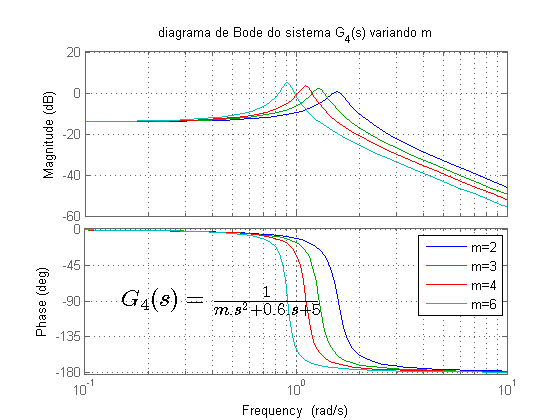
\includegraphics[scale=0.55]{img/task_7_07.png}
    \label{f7}
    \begin{flushleft}
        Fonte: Elaboração própria (2018).
    \end{flushleft}
\end{figure}
\\